\FloatBarrier
\section{Single-Spin Control and Exchange Gates}
\label{app:single-spin-control}
\label{chap:operation-calibration}

The drive Hamiltonian in Appendix~\ref{app:spin-driving} and the
exchange interaction in Section~\ref{sec:exchange-virtual-tunneling}
provide the physical controls for single-spin qubits. To implement a
specified gate, their strengths must be related to the applied pulse
amplitudes and durations. This appendix obtains those relations from
spin oscillations, uses them to construct the gates in
Section~\ref{sec:quantum-gates}, and corrects systematic pulse errors.

The preparation and readout needed for those measurements are developed
in Appendices~\ref{app:state-preparation} and~\ref{app:spin-readout}.
Voltage compensation is treated in Appendix~\ref{app:virtual-gates}.

\subsection{Single-qubit gates for single-spin qubits}
\label{sec:gate-calibration}
\label{sec:time-domain-spin-measurements}
\label{sec:spin-spectroscopy-dynamics}
\label{sec:measurement-zeeman-dynamics}

One electron in one dot stores the logical states
$\ket0=\ket{\downarrow}$ and $\ket1=\ket{\uparrow}$. A static
longitudinal field defines their splitting, while a driven transverse
field supplies logical $x$ and $y$ rotations. Here resonance and rotation-rate
measurements set the pulse parameters for one-qubit gates; repeated
pulse sequences then reveal reproducible angle and axis errors.

\subsubsection{Measuring the resonance and rotation rate}
\label{sec:measurement-spin-spectroscopy}
\label{sec:measurement-rabi}

We use the rotating-frame Hamiltonian in
Eq.~\eqref{eq:logical-phase-drive}. During each rectangular pulse
of duration $\tau$, the drive has a constant amplitude
$\Omega(t)=\Omega_0>0$ and phase $\phi=0$, giving
\begin{equation}
 H_{\mathrm{rot,q}}=\frac{\hbar}{2}(\Omega_0X-\delta Z),
 \qquad \delta=\frac{E_Z}{\hbar}-\omega.
 \label{eq:measurement-rabi-hamiltonian}
\end{equation}
Here $\omega$ is the drive angular frequency.

At fixed amplitude, scanning the drive frequency determines the
resonance; varying the pulse duration at that resonance then
determines the rotation rate. In both scans, prepare $\ket0$,
apply the drive while the
electron remains isolated, and use the single-spin readout of
Section~\ref{sec:calibration-single-spin-readout}. The fraction
of temporary empty-dot records estimates $P_1=P_\uparrow$,
with the assignment correction of
Eq.~\eqref{eq:calibration-assignment-map} when its errors are known.

When decoherence during $\tau$ is negligible, the identity
\[
 (\Omega_0X-\delta Z)^2=(\Omega_0^2+\delta^2)I
\]
gives the propagator
\[
 U(\tau)=\cos\frac{\Omega_{\mathrm{eff}}\tau}{2}I
 -i\sin\frac{\Omega_{\mathrm{eff}}\tau}{2}
       \frac{\Omega_0X-\delta Z}{\Omega_{\mathrm{eff}}}.
\]
Here $\Omega_{\mathrm{eff}}=\sqrt{\Omega_0^2+\delta^2}$.
Starting from $\ket0$ therefore gives
\begin{equation}
 P_\uparrow(\omega,\tau)
 =\frac{\Omega_0^2}{\Omega_0^2+\delta^2}
       \sin^2\!\left(\frac{\sqrt{\Omega_0^2+\delta^2}}{2}\tau\right).
 \label{eq:measurement-rabi-signal}
\end{equation}
Repeat the full preparation--drive--readout cycle at each chosen
frequency and duration, as in
Section~\ref{sec:measurement-pulse-cycle}.

\paragraph{Scanning frequency to measure the spin splitting.}
Keep the holding voltages, $B$, pulse amplitude and $\tau$ fixed
while scanning $\omega$ over a range in which $\Omega_0$ can be treated
as constant. Choose $\tau$ so that
$0<\Omega_0\tau\ll\pi$, so that the resonant response remains far
from the later Rabi maxima and nodes. Under this condition,
Eq.~\eqref{eq:measurement-rabi-signal}, with
$\delta=\omega_{\mathrm{res}}-\omega$, has a central maximum at
$\delta=0$. Measure $P_\uparrow$ at each $\omega$; the location of
that maximum gives $\omega_{\mathrm{res}}$, which obeys
\begin{equation}
 \hbar\omega_{\mathrm{res}}=E_Z=g_{\mathrm e}\mu_BB.
 \label{eq:measurement-spin-resonance-energy}
\end{equation}
It therefore gives $E_Z$; for known $B$, it also gives
$g_{\mathrm e}=\hbar\omega_{\mathrm{res}}/(\mu_BB)$~\cite{Kawakami2014}.

Figure~\ref{fig:calibration-spin-frequency-scan} shows one example
calculated directly from Eq.~\eqref{eq:measurement-rabi-signal}.
It uses the fixed pulse area $\Omega_0\tau=0.5$ and plots the
measured probability against the dimensionless frequency offset
$(\omega-\omega_{\mathrm{res}})\tau$. The central peak occurs at
zero offset, so its horizontal position identifies
$\omega_{\mathrm{res}}$.

\begin{figure}[htbp]
 \centering
 % Exact single-spin frequency response from Eq. (4.8).
% The horizontal coordinate is x=(omega-omega_res)*tau and the
% fixed pulse area is alpha=Omega_0*tau=0.5.
\begingroup
\definecolor{spinScanBlue}{HTML}{0072B2}
\pgfmathdeclarefunction{spinScanProbability}{1}{%
 \pgfmathparse{0.25/(0.25+#1*#1)*%
   sin(deg(0.5*sqrt(0.25+#1*#1)))^2}%
}
\begin{tikzpicture}[
 x=4.4mm,y=500mm,>=stealth,line cap=round,line join=round,
 every node/.style={font=\small,inner sep=1.5pt}
]
 \path[use as bounding box] (-14,-0.017) rectangle (14,0.082);

 \draw[->,line width=0.45pt] (-12,0)--(12.8,0);
 \draw[->,line width=0.45pt] (-12,0)--(-12,0.074);
 \node[anchor=west] at (12.8,-0.008)
      {$(\omega-\omega_{\mathrm{res}})\tau$};
 \node[anchor=south] at (-12,0.074) {$P_\uparrow$};

 \foreach \x in {-10,-5,0,5,10}{
  \draw[line width=0.35pt] (\x,0)--(\x,-0.0015);
  \node[anchor=north] at (\x,-0.002) {$\x$};
 }
 \foreach \y/\labeltext in {0.02/{0.02},0.04/{0.04},0.06/{0.06}}{
  \draw[line width=0.35pt] (-12,\y)--(-12.18,\y);
  \node[anchor=east] at (-12.25,\y) {$\labeltext$};
 }

 \draw[black!35,dash pattern=on 2pt off 1.5pt,line width=0.45pt]
       (0,0)--(0,{spinScanProbability(0)});
 \draw[spinScanBlue,line width=0.9pt]
       plot[domain=-12:12,samples=401]
       (\x,{spinScanProbability(\x)});
 \fill[spinScanBlue] (0,{spinScanProbability(0)}) circle[radius=0.55mm];
 \node[anchor=south west] at (0.5,0.061)
       {$\omega=\omega_{\mathrm{res}}$};
\end{tikzpicture}
\endgroup

 \caption{Example frequency scan from the exact two-level result
 in Eq.~\eqref{eq:measurement-rabi-signal}, for
 $\Omega_0\tau=0.5$ and negligible decoherence. The vertical axis
 is the actual spin-up probability, not a normalized line shape.
 The dashed line marks the resonant angular frequency. This is a
 theoretical example, not experimental data.}
 \label{fig:calibration-spin-frequency-scan}
\end{figure}

\paragraph{Scanning duration to measure the rotation rate.}
Now fix $\omega=\omega_{\mathrm{res}}$ and keep the amplitude constant
while varying $\tau$. At $\delta=0$,
\begin{equation}
 P_\uparrow(\omega_{\mathrm{res}},\tau)
       =\sin^2\!\left(\frac{\Omega_0\tau}{2}\right),
 \qquad \tau_\pi=\frac{\pi}{\Omega_0}.
 \label{eq:measurement-resonant-rabi}
\end{equation}
The oscillation period is $2\pi/\Omega_0$, and the first maximum
gives the spin-flip time $\tau_\pi$. At each duration, count the up-spin outcomes
in repeated trials and fit the probability-versus-duration curve
to determine $\Omega_0$.

The measured rotation rate includes the device response and the
attenuation between generator and gate for the applied pulse.
Repeating at nearby frequencies checks the detuning dependence:
the oscillation becomes faster but its maximum transfer becomes
smaller away from resonance. Contrast decay during driving can
also contain relaxation, fluctuations and pulse errors.

\subsubsection{Implementing single-spin gates with calibrated pulses}
\label{sec:calibration-spin-rotations}

The preceding scan calibrates the constant strength $\Omega_0$.
To turn that calibrated evolution into a gate, use the rectangular
drive envelope
\[
 \Omega(t)=
 \begin{cases}
  \Omega_0,&0<t<t_p,\\
  0,&\text{otherwise}.
 \end{cases}
\]
Retain the holding voltages and amplitude used in the calibration,
choose the transverse axis through the drive phase, and choose the
pulse duration $t_p$ to obtain the required rotation angle.

Set $\omega=\omega_{\mathrm{res}}=E_Z/\hbar$, so $\delta=0$.
The constant Hamiltonian gives
\[
 U(t_p)=U_\phi(\vartheta)
 =\exp\!\left[-\frac{i\vartheta}{2}
                   (\cos\phi X-\sin\phi Y)\right],
 \qquad \vartheta=\Omega_0t_p.
\]
For a desired angle $\theta>0$, choose
\[
 \begin{array}{c|c|c}
 \text{target rotation}&\phi&t_p\\ \hline
 R_x(\theta)&0&\theta/\Omega_0\\
 R_y(\theta)&-\pi/2&\theta/\Omega_0\\
 R_x(-\theta)&\pi&\theta/\Omega_0\\
 R_y(-\theta)&+\pi/2&\theta/\Omega_0
 \end{array}
\]
Thus $R_x(\pi/2)$ uses phase zero and duration $\pi/(2\Omega_0)$,
while $R_x(\pi)$ uses the same phase and duration $\pi/\Omega_0$.
The holding voltages and applied amplitude remain those used in the
measurement of $\Omega_0$. Successive pulses share the same
oscillating phase reference.

\paragraph{Executing the pulse and checking its angle.}
To test the prescribed $x$ rotation, prepare down, move to the
holding voltages, and apply the rectangular pulse just specified.
Then turn the drive off, move to the fixed readout voltages, and
repeat this full sequence. The up-spin fraction, corrected for
known assignment errors, estimates
\[
 P_1=\left|\bra1 R_x(\theta)\ket0\right|^2
    =\sin^2(\theta/2).
\]
For the $\pi/2$ and $\pi$ pulses this predicts $1/2$ and $1$.
If the holding voltages or delivered amplitude have changed since
the Rabi measurement, first update $\Omega_0$ with a duration scan.

\paragraph{Including fixed pulse edges.}
A finite pulse also rotates the spin while its amplitude rises and
falls. At resonance and fixed phase, the angle remains the integral
of $\Omega(t)$. Consider a pulse with a constant plateau $\Omega_0>0$
of adjustable duration $t_{\mathrm h}$ and fixed edges. If changing
$t_{\mathrm h}$ leaves the edge waveforms unchanged, write their
combined area as $\vartheta_{\mathrm{edge}}$. The full angle and the
ideal probability measured from $\ket0$ are then
\begin{equation}
 \vartheta(t_{\mathrm h})
    =\vartheta_{\mathrm{edge}}+\Omega_0t_{\mathrm h},\qquad
 P_1(t_{\mathrm h})
    =\sin^2\!\left(\frac{\vartheta_{\mathrm{edge}}
                              +\Omega_0t_{\mathrm h}}{2}\right).
 \label{eq:calibration-drive-edge-area}
\end{equation}
Keep the programmed amplitude, phase and edges fixed, vary only
the plateau duration, and measure $P_1$ using the same preparation
and readout as above. The oscillation period determines $\Omega_0$,
while its phase offset determines $\vartheta_{\mathrm{edge}}$ modulo
$2\pi$. For a target angle $\vartheta^\star$, choose
\begin{equation}
 t_{\mathrm h}
   =\frac{\vartheta^\star-\vartheta_{\mathrm{edge}}+2\pi m}{\Omega_0},
 \qquad m\in\mathbb Z,
 \label{eq:calibration-drive-hold-duration}
\end{equation}
with a branch that gives an allowed positive hold time. Repeat this
area calibration when the applied amplitude or edge waveform is
changed. These relations use the same negligible-decoherence limit
as the rectangular-pulse calculation; a pulse whose phase or
detuning changes must be treated with its full Hamiltonian.

This pulse prescription fixes the ideal driven rotation. The next
subsection corrects reproducible angle and axis errors before the
operation is tested on several inputs in
Appendix~\ref{app:gate-verification}.

\subsubsection{Correcting systematic pulse errors}
\label{sec:calibration-spin-corrections}

The resonance and Rabi scans provide initial settings for the drive
frequency, amplitude and duration. We now amplify small,
reproducible discrepancies between the intended and actual pulse.
An amplitude or duration error changes the rotation angle; a
frequency error adds a $Z$ component to the rotation axis; and a
relative-phase error rotates the intended transverse axis within
the $xy$ plane. The three tests below determine which control must
be corrected.

\paragraph{Detecting whether a pulse rotates too far or not far enough.}
Start with a nominal $R_x(\pi)$ pulse. A single measurement near its
maximum transfer is insensitive to the sign of a small angle error.
Repeating the pulse lets the error accumulate; an extra $\pi/2$
pulse places the final probability on a slope where its sign is visible.

If a nominal $R_x(\pi)$ is actually $R_x(\pi+\eta)$ and other
errors are negligible, $m$ repetitions give
\begin{equation}
 P_1(m)=\sin^2\!\left[\frac{m(\pi+\eta)}2\right].
 \label{eq:calibration-angle-amplification}
\end{equation}
Thus an error hidden in one pulse becomes a visible modulation as
$m$ increases. Scan the pulse amplitude or duration around the
initial estimate, record this dependence, and find the setting
consistent with $\eta=0$ for several $m$. Population data of this
form alone do not determine the sign of $\eta$.

To obtain a signed correction, take even $m$ and append an
$R_x(\pi/2)$ analysis pulse before readout. The ideal repeated
$\pi$ pulses now give $P_1=1/2$, on the slope rather than the
extremum of the oscillation:
\begin{equation}
 P_1^{\mathrm{quad}}(m)
 =\sin^2\left(\frac{m(\pi+\eta)+\pi/2}{2}\right)
 =\frac{1+\sin(m\eta)}2
 \simeq\frac12+\frac{m\eta}{2}.
 \label{eq:calibration-signed-angle-error}
\end{equation}
In the range $|m\eta|\ll1$, a measured deviation from $1/2$ gives
$\eta\simeq2(P_1^{\mathrm{quad}}-1/2)/m$, including its sign.
An analysis-pulse angle error adds an intercept independent of
$m$; measuring several even $m$ separates that intercept from
the slope. If the adjustable control is the rectangular amplitude
$a_0$ and its measured angle slope is $s_a=d\vartheta/da_0$,
change $a_0$ by $-\eta/s_a$. Repeating the sequence verifies the correction.
All probabilities here refer to assignment-corrected counts.

\paragraph{Correcting the drive frequency from an axis error.}
Even a correct pulse area fails to give a pure $x$ rotation if
$\omega\ne E_Z/\hbar$. The term $-\hbar\delta Z/2$ tilts its axis
towards $z$. A nominal $\pi$ pulse then leaves a transverse spin
component whose sign reveals the sign of the detuning.
For a rectangular pulse with constant Rabi frequency $\Omega_0$
and phase zero, define
$\Omega_{\mathrm{eff}}=\sqrt{\Omega_0^2+\delta^2}$.
The propagator is
\[
 U(t)=\cos\frac{\Omega_{\mathrm{eff}}t}{2}I
 -i\sin\frac{\Omega_{\mathrm{eff}}t}{2}
                 \frac{\Omega_0 X-\delta Z}{\Omega_{\mathrm{eff}}}.
\]
Starting in $\ket0$, its output satisfies
\begin{equation}
 \begin{aligned}
 P_1(t)&=\frac{\Omega_0^2}{\Omega_0^2+\delta^2}
                  \sin^2\frac{\Omega_{\mathrm{eff}}t}{2},\\
 \langle X\rangle(t)&=
  -\frac{\Omega_0\delta}{\Omega_0^2+\delta^2}
                     [1-\cos(\Omega_{\mathrm{eff}}t)].
 \end{aligned}
 \label{eq:calibration-axis-error-signal}
\end{equation}
At the nominal $\pi$ time $\pi/\Omega_0$ and small detuning,
$\langle X\rangle\simeq-2\delta/\Omega_0$. Unlike the population
deficit, this is linear in the detuning and reveals its sign.
Measure it by adding $R_y(-\pi/2)$ before logical-basis readout,
then update the reference frequency by $\omega\mapsto\omega+\delta$.
The analysis pulse must have independently established phase and
small axis error. The resonance scan supplies the initial frequency
setting, and the signed axis-error signal above supplies its local
correction. The Ramsey fringe-phase slope in
Section~\ref{sec:measurement-ramsey-echo} independently shows any
residual mean detuning during a wait. Amplitude and frequency updates
can be alternated until both signed signals vanish within the chosen
accuracy.

\paragraph{Checking the relative transverse axes of two pulses.}
A population measurement after one $\pi/2$ pulse cannot distinguish
an $x$ rotation from a $y$ rotation: both give $P_1=1/2$ from
$\ket0$. A second pulse makes their relative axis observable
through interference.
Apply $R_x(\pi/2)$ followed immediately by a second $\pi/2$ pulse
with phase $\phi$. Using Eq.~\eqref{eq:calibration-single-spin-hamiltonian}
at $\delta=0$ gives
\begin{equation}
 P_1(\phi)
 =\left|\bra1 U_\phi(\pi/2)R_x(\pi/2)\ket0\right|^2
 =\frac{1+\cos\phi}{2}.
 \label{eq:calibration-drive-phase}
\end{equation}
Scan the programmed relative phase and find its offset from this
curve. The same phase reference must be maintained between pulses.
This establishes relative axes; the choice of what is called the
$x$ axis fixes their common phase convention.

These tests return corrections to duration or amplitude, reference
frequency, and relative phase, respectively. After a correction,
repeat the associated test at the same holding voltages. Random
changes between repetitions are not fixed pulse missettings. Their
effect during a wait is measured in
Section~\ref{sec:idle-single-spin-characterization}, while their
effect during a gate is treated in
Appendix~\ref{app:noise-leakage}.

\subsection{Two-qubit gates for single-spin qubits}
\label{sec:measurement-exchange-oscillations}

During an exchange pulse, the two basis states with opposite spins
are $\ket{01}=\ket{\downarrow\uparrow}$ and
$\ket{10}=\ket{\uparrow\downarrow}$. After removing a scalar energy,
their dynamics is governed by
\begin{equation}
 H_{0}(t)=
 \begin{pmatrix}
  -\Delta E_Z/2 & J(t)/2\\
  J(t)/2 & +\Delta E_Z/2
 \end{pmatrix},
 \qquad \Delta E_Z=E_{Z,1}-E_{Z,2}.
 \label{eq:calibration-two-spin-subspace-hamiltonian}
\end{equation}
The diagonal term is the difference between the two local Zeeman
splittings. The off-diagonal term converts $\ket{01}$ into
$\ket{10}$ and vice versa; it is the part used to exchange the two
spin states. A SWAP-type gate therefore requires a controlled
$J(t)$ and either negligible $\Delta E_Z$ during the pulse or an
explicit treatment of its simultaneous evolution.

The coupling $J(t)$ is produced by lowering the interdot barrier.
This increases tunneling, and virtual double occupation produces
the exchange Hamiltonian
\begin{equation}
 H_{\mathrm{ex}}(t)=J(t)\,\mathbf s_1\cdot\mathbf s_2,
 \qquad \mathbf s_i=\boldsymbol{\sigma}_i/2.
 \label{eq:measurement-exchange-hamiltonian}
\end{equation}
Exchange changes the relative phase of the singlet and triplet
components of a two-spin state. We first estimate its scale from a
virtual-tunneling model, then calibrate the effective $J$ from the
measured spin oscillation. The calibrated pulse area sets SWAP and
$\sqrt{\mathrm{SWAP}}$ gates. A composite sequence combines the same
interaction with local single-spin rotations to obtain a diagonal
entangling gate.

\subsubsection{Estimating the exchange scale from virtual tunneling}
\label{sec:calibration-exchange-estimate}

The device model gives an initial estimate of the exchange coupling
that can be used to choose a safe range of barrier amplitudes and
pulse durations for the first experiment. Lowering the interdot
barrier increases the tunneling amplitude $t_c$. The higher-energy
$(2,0)$ and $(0,2)$ configurations then contribute virtually: in a
single-orbital model they lower the singlet energy but not the
triplet energy.
Let $\ket{S_{11}}$ be the separated singlet and let
$\ket{S_{20}}$ and $\ket{S_{02}}$ be the doubly occupied singlets.
Define their positive energy costs relative to $\ket{S_{11}}$ by
\[
 \Delta_{20}=E(S_{20})-E(S_{11}),\qquad
 \Delta_{02}=E(S_{02})-E(S_{11}).
\]
Single-electron tunneling couples $\ket{S_{11}}$ to each doubly
occupied singlet with matrix-element magnitude $\sqrt2t_c$.
For $\Delta_{20},\Delta_{02}\gg |t_c|$, second-order perturbation
theory therefore gives
\[
 \delta E_S=-\frac{2t_c^2}{\Delta_{20}}
             -\frac{2t_c^2}{\Delta_{02}}.
\]
The corresponding triplets cannot put two electrons into the same
single-dot orbital, so they have no such second-order shift in this
single-orbital model. The singlet--triplet splitting is consequently
\[
 J=E_T-E_S\simeq
 2t_c^2\left(\frac1{\Delta_{20}}+\frac1{\Delta_{02}}\right),
 \qquad H_{\mathrm{ex}}=J\,\mathbf s_1\cdot\mathbf s_2,
 \qquad \mathbf s_i=\boldsymbol\sigma_i/2.
\]
This expression estimates the scale and voltage dependence of $J$
within the single-orbital, second-order model. The value used to set
a gate is instead obtained from the exchange-oscillation experiment
below.
This is the virtual-charge mechanism introduced more briefly in
Section~\ref{sec:exchange-virtual-tunneling}.

\subsubsection{Calibrating exchange from spin oscillations}
\label{sec:calibration-two-spin-exchange}
\label{sec:measurement-two-spin-exchange}

Experimentally, $J$ is changed by applying voltages to the electrode
above the interdot barrier. A voltage on that electrode also shifts
the two dot energies, so two compensating plunger-voltage changes are
applied at the same time. Collect the physical electrode voltages as
$\mathbf V=(V_1,V_2,V_{\mathrm B})^T$ and write the coordinated pulse as
\begin{equation}
 \mathbf V(t)=\mathbf V^0+\mathbf n v(t),\qquad
 \mathbf n=(n_1,n_2,1)^T,\qquad G\mathbf n=0.
 \label{eq:calibration-exchange-voltage-pulse}
\end{equation}
Here $v(t)$ is the applied barrier-voltage increment, while $n_1v(t)$
and $n_2v(t)$ are the simultaneous plunger corrections. The condition
$G\mathbf n=0$ keeps the two addition energies fixed to first order,
as derived in Appendix~\ref{app:virtual-gates}.

Choose the sign of $v$ so that increasing its pulse amplitude lowers
the potential barrier between the dots. The orbital overlap and
$t_c$ then increase, so the estimate in
Section~\ref{sec:calibration-exchange-estimate} predicts a larger
$J$. This prediction gives only the direction and scale of the
change: the function $J(v)$ is determined experimentally by the
duration scan below. During every pulse, keep the two reservoir
barriers closed so that the electron number remains fixed; ramp from
$v=0$ to a chosen amplitude, hold, and return to $v=0$ before readout.

\begin{figure}[htbp]
 \centering
 % Schematic compensated barrier pulse and the resulting exchange response.
\begingroup
\definecolor{exchangePulseBlue}{HTML}{0072B2}
\definecolor{exchangePulseOrange}{HTML}{D55E00}
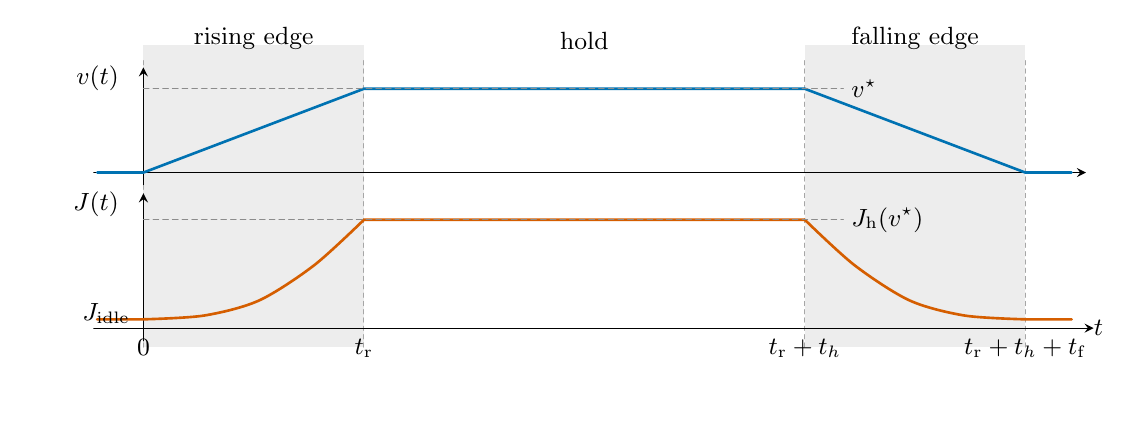
\begin{tikzpicture}[
 x=14mm,y=8mm,>=stealth,line cap=round,line join=round,
 every node/.style={font=\small,inner sep=1.5pt}
]
 \path[use as bounding box] (-1.05,-0.45) rectangle (8.85,5.35);

 % The two shaded intervals are the pulse edges.
 \fill[black!7] (0,0.28) rectangle (2,5.08);
 \fill[black!7] (6,0.28) rectangle (8,5.08);
 \node[anchor=south] at (1,4.93) {rising edge};
 \node[anchor=south] at (4,4.93) {hold};
 \node[anchor=south] at (7,4.93) {falling edge};

 % Shared switching times.
 \foreach \x in {0,2,6,8}{
  \draw[black!35,dash pattern=on 1.5pt off 1.5pt,line width=0.4pt]
       (\x,0.28)--(\x,4.88);
 }

 % Applied compensated-barrier coordinate v(t).
 \draw[->,line width=0.45pt] (-0.45,3.05)--(8.55,3.05);
 \draw[->,line width=0.45pt] (0,2.86)--(0,4.72);
 \node[anchor=east] at (-0.18,4.55) {$v(t)$};
 \draw[exchangePulseBlue,line width=0.95pt]
       (-0.42,3.05)--(0,3.05)--(2,4.38)--(6,4.38)--(8,3.05)--(8.42,3.05);
 \draw[black!45,dash pattern=on 2pt off 1.5pt,line width=0.4pt]
       (0,4.38)--(6.35,4.38);
 \node[anchor=west] at (6.38,4.38) {$v^\star$};

 % Exchange coupling J(t).  Curved edges emphasize J's nonlinear voltage response.
 \draw[->,line width=0.45pt] (-0.45,0.58)--(8.62,0.58);
 \draw[->,line width=0.45pt] (0,0.38)--(0,2.72);
 \node[anchor=east] at (-0.18,2.55) {$J(t)$};
 \draw[exchangePulseOrange,line width=0.95pt]
       (-0.42,0.72)--(0,0.72)
       plot[smooth] coordinates {(0,0.72) (0.55,0.78) (1.05,1.02) (1.55,1.58) (2,2.30)}
       --(6,2.30)
       plot[smooth] coordinates {(6,2.30) (6.45,1.58) (6.95,1.02) (7.45,0.78) (8,0.72)}
       --(8.42,0.72);
 \draw[black!45,dash pattern=on 2pt off 1.5pt,line width=0.4pt]
       (0,2.30)--(6.35,2.30);
 \node[anchor=west] at (6.38,2.30) {$J_{\mathrm h}(v^\star)$};
 \node[anchor=east] at (-0.08,0.82) {$J_{\mathrm{idle}}$};

 % Time labels.
 \node[anchor=north] at (0,0.48) {$0$};
 \node[anchor=north] at (2,0.48) {$t_{\mathrm r}$};
 \node[anchor=north] at (6,0.48) {$t_{\mathrm r}+t_h$};
 \node[anchor=north] at (8,0.48) {$t_{\mathrm r}+t_h+t_{\mathrm f}$};
 \node[anchor=west] at (8.58,0.58) {$t$};
\end{tikzpicture}
\endgroup

 \caption{A compensated barrier pulse and the resulting exchange
 coupling. The programmed coordinate $v(t)$ rises from zero to
 $v^\star$, remains there for the hold time $t_h$, and returns to
 zero. All physical gate voltages follow
 $\mathbf V(t)=\mathbf V^0+\mathbf n v(t)$. The exchange response
 $J(t)$ need not have linear edges because $J$ is generally a
 nonlinear function of voltage. The shaded rising and falling
 intervals together produce the edge phase
 $\theta_{\mathrm{edge}}$; the flat interval contributes
 $J_{\mathrm h}t_h/\hbar$.}
 \label{fig:calibration-exchange-pulse-shape}
\end{figure}

\paragraph{Evolution of two opposite spins.}
Figure~\ref{fig:calibration-exchange-pulse-shape} divides the pulse
into a rise of duration $t_{\mathrm r}$, a flat hold of duration
$t_h$, and a fall of duration $t_{\mathrm f}$. During the hold,
$v(t)=v^\star$ and $J(t)=J_{\mathrm h}(v^\star)$ are constant.
The complete exchange angle is
\begin{equation}
 \begin{aligned}
 \theta
 &=\frac1\hbar
   \int_0^{t_{\mathrm r}+t_h+t_{\mathrm f}}J(t)\,dt\\
 &=\underbrace{\frac1\hbar
   \left[
    \int_0^{t_{\mathrm r}}J(t)\,dt+
    \int_{t_{\mathrm r}+t_h}^{t_{\mathrm r}+t_h+t_{\mathrm f}}
            J(t)\,dt
   \right]}_{\displaystyle\theta_{\mathrm{edge}}}
   +\frac{J_{\mathrm h}(v^\star)t_h}{\hbar}.
 \end{aligned}
 \label{eq:calibration-exchange-pulse-area}
\end{equation}
Thus \emph{edge} denotes both nonflat parts of the pulse together,
not an additional Hamiltonian term. The singlet and triplets have
exchange energies $-3J/4$ and $J/4$, so $\theta$ is their accumulated
relative phase.

For two single-spin qubits, prepare
$\ket{01}=\ket{\downarrow\uparrow}=(\ket{T_0}-\ket S)/\sqrt2$.
The ideal exchange formula below assumes that $\Delta E_Z$ is
negligible during the pulse or that its known evolution is canceled
by a refocusing sequence. This is the condition stated in the
introductory gate discussion of
Section~\ref{sec:exchange-two-qubit-gates}; it is repeated here
because it determines the measured oscillation. Under this condition,
exchange produces
\[
 \ket{01}\longmapsto
 e^{i\theta/4}
 \left[\cos(\theta/2)\ket{01}-i\sin(\theta/2)\ket{10}\right].
\]
For this test input, the exchanged-state probability is
\begin{equation}
 P_{10}=\sin^2(\theta/2).
 \label{eq:calibration-exchange-area}
\end{equation}

\paragraph{Measuring the coupling from the oscillation.}
Choose one barrier-pulse amplitude and keep its rising and falling
edges fixed, so $\theta_{\mathrm{edge}}$ is the same in every trial.
Vary only the flat hold time $t_h$. If $\Delta E_Z$ is negligible,
Eqs.~\eqref{eq:calibration-exchange-pulse-area} and
\eqref{eq:calibration-exchange-area} predict
\begin{equation}
 P_{10}(t_h)=
 \sin^2\!\left(\frac{\theta_{\mathrm{edge}}}{2}
                +\frac{J_{\mathrm h}t_h}{2\hbar}\right).
 \label{eq:calibration-exchange-duration-scan}
\end{equation}
The barrier pulse therefore moves the state repeatedly between
$\ket{01}$ and $\ket{10}$. Increasing $t_h$ does not change the
Hamiltonian during the hold; it only lets the same Hamiltonian act
for longer.

For each chosen $t_h$, initialize both spins down and flip the
second spin using Section~\ref{sec:calibration-spin-rotations} to
prepare $\ket{01}$. Apply the barrier pulse, return to the
weak-exchange setting, and read the two spins separately using
Section~\ref{sec:calibration-single-spin-readout}. Repeat the full
sequence many times. The assignment-corrected fraction of
$\ket{10}$ outcomes estimates $P_{10}(t_h)$. Repeating this procedure
for a set of hold times produces the exchange-oscillation curve.

Fit that curve to
Eq.~\eqref{eq:calibration-exchange-duration-scan}. Its horizontal
period $T_{\mathrm{ex}}$ satisfies
\begin{equation}
 \frac{J_{\mathrm h}T_{\mathrm{ex}}}{2\hbar}=\pi,
 \qquad
 J_{\mathrm h}=\frac{2\pi\hbar}{T_{\mathrm{ex}}}
              =\frac{h}{T_{\mathrm{ex}}}.
 \label{eq:calibration-exchange-from-period}
\end{equation}
The horizontal offset determines $\theta_{\mathrm{edge}}$ modulo
$2\pi$; it does not change the period. A measured contrast below
one can arise from preparation and readout errors, dephasing, or a
nonzero $\Delta E_Z$, but it does not by itself change the ideal
period-to-$J_{\mathrm h}$ conversion when $\Delta E_Z$ is negligible.

If $\Delta E_Z$ cannot be neglected, the flat-hold Hamiltonian is
the matrix in
Eq.~\eqref{eq:calibration-two-spin-subspace-hamiltonian}. Since
\[
 H_0^2=\frac{J_{\mathrm h}^2+\Delta E_Z^2}{4}I,
\]
an ideal rectangular hold starting from $\ket{01}$ gives
\begin{equation}
 P_{10}(t_h)=
 \frac{J_{\mathrm h}^2}{J_{\mathrm h}^2+\Delta E_Z^2}
 \sin^2\!\left(
  \frac{\sqrt{J_{\mathrm h}^2+\Delta E_Z^2}}{2\hbar}t_h
 \right).
 \label{eq:calibration-exchange-gradient-scan}
\end{equation}
The Zeeman difference therefore both reduces the maximum transfer
and increases the oscillation frequency. Use an independently
measured $\Delta E_Z$ when fitting this expression; otherwise an
imperfect readout contrast can be confused with the prefactor above.
Fixed noninstantaneous pulse edges can instead be included by
propagating the full measured waveform.

Finally, repeat the duration scan at several points
$\mathbf V(v)=\mathbf V^0+\mathbf n v$ on the compensated voltage
path. The fitted value at each point gives the required response
$J_{\mathrm h}(v)$.

\subsubsection{Choosing the amplitude and duration of a partial-SWAP pulse}
\label{sec:calibration-partial-swap}

The preceding subsection supplies two measured quantities for each
barrier-pulse amplitude $v$: the flat-hold coupling $J_{\mathrm h}(v)$
and the phase $\theta_{\mathrm{edge}}(v)$ accumulated on the fixed
rising and falling edges. We now convert a target exchange gate into
the two pulse settings that the control system needs: an amplitude
$v^\star$ and a hold time $t_h$.

Assume first that $\Delta E_Z$ is negligible or refocused. The
complete pulse then implements
\begin{equation}
 U_{\mathrm{ex}}(\theta)
 =\exp[-i\theta\,\mathbf s_1\cdot\mathbf s_2],\qquad
 \theta(v,t_h)=\theta_{\mathrm{edge}}(v)
                 +\frac{J_{\mathrm h}(v)t_h}{\hbar}.
 \label{eq:calibration-complete-exchange-pulse}
\end{equation}
The family is called partial-SWAP because varying $\theta$ continuously
changes how much of $\ket{01}$ is transferred to $\ket{10}$.
The choices $\theta^\star=\pi$ and $\theta^\star=\pi/2$ give SWAP and
$\sqrt{\mathrm{SWAP}}$, respectively, up to a common phase.

Choose an amplitude $v^\star$ inside the range already tested by the
duration scans. The corresponding hold time is
\begin{equation}
 t_h=
 \frac{\hbar[
   \theta^\star-\theta_{\mathrm{edge}}(v^\star)+2\pi m]}
      {J_{\mathrm h}(v^\star)},
 \qquad m\in\mathbb Z,
 \label{eq:calibration-partial-swap-duration}
\end{equation}
where the integer $m$ selects a branch with an allowed positive
duration. If $v^\star$ lies between measured amplitudes, interpolate
both measured functions $J_{\mathrm h}(v)$ and
$\theta_{\mathrm{edge}}(v)$; do not extrapolate beyond the calibrated
voltage interval.

Prepare $\ket{01}$ and apply the selected pulse. The expected
population check is
\[
 P_{10}=\sin^2(\theta^\star/2),
\]
which equals $1$ for SWAP and $1/2$ for $\sqrt{\mathrm{SWAP}}$.
This check verifies the exchange area for that input. The
multi-input tests in Appendix~\ref{app:gate-verification}
are still required to verify the complete gate, including its
relative phases. If $\Delta E_Z$ is appreciable and not refocused,
the pulse implements evolution under the full $H_0$ rather than a
pure partial-SWAP; its amplitude and duration must then be chosen
from that full propagator.


\subsubsection{Constructing CZ from exchange and local rotations}
\label{sec:calibration-single-spin-exchange-cz}

A single isotropic exchange pulse contains
$X_AX_B$, $Y_AY_B$ and $Z_AZ_B$ with the same coefficient. It
therefore produces a partial SWAP rather than a diagonal
controlled-phase gate. Local $z$ rotations can reverse the first
two products without reversing the third, allowing two exchange
pulses to retain only the $Z_AZ_B$ interaction.

Let
\[
 G=\exp\!\left[-\frac{i\pi}{8}
  (X_AX_B+Y_AY_B+Z_AZ_B)\right]
\]
be the exchange gate with area $\theta=\pi/2$, calibrated by the
oscillation measurement above. Conjugation by $Z_A$ reverses
$X_AX_B$ and $Y_AY_B$ but leaves $Z_AZ_B$ unchanged. Since the
three Pauli products commute,
\begin{equation}
 GZ_AGZ_A=\exp(-i\pi Z_AZ_B/4).
 \label{eq:calibration-exchange-zz-repeated}
\end{equation}
This is the exchange construction introduced in
Eq.~\eqref{eq:exchange-zz-construction}, now written in terms of
the pulses calibrated in
Section~\ref{sec:calibration-spin-rotations}. The remaining local phases
are removed by
\begin{equation}
 \mathrm{CZ}
 =e^{-i\pi/4}R_{z,A}(-\pi/2)R_{z,B}(-\pi/2)
       \exp(-i\pi Z_AZ_B/4).
 \label{eq:calibration-single-spin-cz}
\end{equation}

The exchange area and the local rotations are first set by their
individual calibrations, but the conditional phase of the complete
sequence must also be measured. Prepare qubit $A$ in
$\ket+=(\ket0+\ket1)/\sqrt2$ and qubit $B$ in $\ket b$, with
$b=0$ and $1$ in separate repetitions. If the complete diagonal
sequence gives phases $\chi_{ab}$, the relative phase observed on
$A$ is $d_b=\chi_{1b}-\chi_{0b}$. Analysis rotations before
logical-basis readout determine both $\cos d_b$ and $\sin d_b$.
The nonlocal phase is
\begin{equation}
 \Theta=d_1-d_0
 =\chi_{11}-\chi_{10}-\chi_{01}+\chi_{00}.
 \label{eq:calibration-single-spin-conditional-phase}
\end{equation}
Adjust the exchange hold durations until
$\Theta=\pi$ modulo $2\pi$, then update the two local $z$ rotations
from the separately measured single-qubit phases. This measurement
calibrates the complete composite gate rather than assuming that
the phases of its component pulses add ideally.
